\documentclass{standalone}
\usepackage{tikz}
\usepackage{tkz-euclide}
\usepackage{ctex}
\setCJKmainfont{Noto Serif CJK SC}
\usepackage{chemfig,siunitx}
\begin{document}
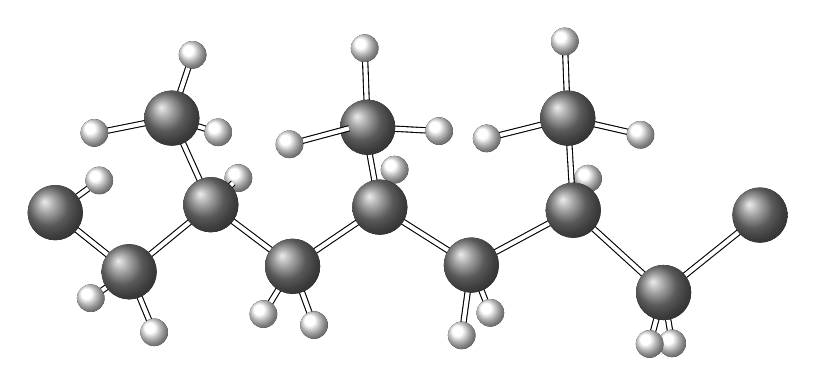
\begin{tikzpicture}[scale=0.7]
  \foreach \x/\y in {
     4.423/4.198,
 7.257/4.350,
10.766/4.187
  }
  { \fill[ball color=white](\x,\y)circle(0.25); }
  \draw[double,double distance=1.5pt](3.21,5.29)--(1.81,5.01);
  \draw[double,double distance=1.5pt](3.21,5.29)--(4.05,5.02);
  \draw[double,double distance=1.5pt](3.21,5.29)--(3.59,6.43);
  \draw[double,double distance=1.5pt](8.065,5.050)--(6.768,5.119)--(6.714,6.554);
  \draw[double,double distance=1.5pt](11.718,4.983)--(10.399,5.285)--(10.345,6.676);
  \draw[double,double distance=1.5pt]( 8.928,4.917)--(10.399,5.285)--(10.498,3.614);
  \draw[double,double distance=1.5pt](13.886,3.526)--(12.137,2.121)--(10.498,3.614)--( 8.650,2.619)--( 6.989,3.670)--( 5.406,2.597)--( 3.923,3.714)--( 2.440,2.497)--( 1.100,3.570)--( 1.899,4.154);
  \draw[double,double distance=1.5pt](8.994,1.753)--(8.650,2.619)--(8.474,1.343);
  \draw[double,double distance=1.5pt](2.895,1.399)--(2.440,2.497)--(1.744,2.018);
  \draw[double,double distance=1.5pt](4.877,1.730)--(5.406,2.597)--(5.795,1.531);
  \draw[double,double distance=1.5pt](11.884,1.188)--(12.137,2.121)--(12.293,1.199);
  \draw[double,double distance=1.5pt](3.923,3.714)--(3.215,5.285);
  % \fill[ball color=white](,)circle(0.25);
  \foreach \x/\y in {
     1.899/4.154,
 1.810/5.017,
 3.592/6.433,
 4.057/5.028,
 6.714/6.554,
 8.065/5.050,
 8.928/4.917,
10.345/6.676,
11.718/4.983,
12.293/1.199,
11.884/1.188,
 8.994/1.753,
 8.474/1.343,
 5.795/1.531,
 4.877/1.730,
 2.895/1.399,
 1.744/2.018
  }
  { \fill[ball color=white](\x,\y)circle(0.25); }
  \draw[double,double distance=1.5pt](4.33,4.11)--(3.92,3.71);
  \draw[double,double distance=1.5pt](6.75,4.93)--(6.98,3.67);
  \foreach \x/\y in {
    13.886/3.526,
    12.137/2.121,
    10.498/3.614,
    8.650/2.619,
    6.989/3.670,
    5.406/2.597,
    3.923/3.714,
    2.440/2.497,
    1.100/3.570,
     3.215/5.285,
 6.768/5.119,
10.399/5.285
  }
  {
    \fill[ball color=gray](\x,\y)circle(0.5);
  }
  \draw[double,double distance=1.5pt](6.43,5.10)--(5.35,4.81);
  \fill[ball color=white](5.35,4.81)circle(0.25);
\end{tikzpicture}
\end{document}